\section{Error Analysis}
This section looks at where the models make their largest mistakes on the test set. All numbers come from \texttt{src/bias\_check.py}, and the tables are saved in the \texttt{results/} folder. Error means predicted minus actual power, so a negative bias means that the model predicts too little.

\subsection{Error by hour of the day}
Figure~\ref{fig:errhour} shows the error for each hour. At night (hours 19 to 5) the output is zero and both models predict almost zero, with an average error of only about 2 to 5. In the daytime the absolute error is largest around midday (hours 11 and 12: MAE about 502 for gradient boosting and 562 to 607 for the neural network), because the output itself is largest then (a mean of about 9,700). As a share of the output, the error at midday is about 5\%. The largest relative errors are at the edges of the day: in the hour starting at 18:00 the error is 10.6\% of the mean output for gradient boosting and 19.1\% for the neural network, and in the hour starting at 06:00 it is 6.0\% and 11.2\%. In absolute terms these errors are small (24 and 43 at 18:00), so they hardly change the daily energy total, which is what the savings estimate uses.

The signed error shows a difference between the models. Gradient boosting has almost no bias at any hour (the largest is $+44$ at hour 9, which is 0.6\% of the mean output of that hour). The neural network predicts too little in every hour from 6 to 18 except noon, by between 1 and 100.

\begin{figure}[H]
\centering
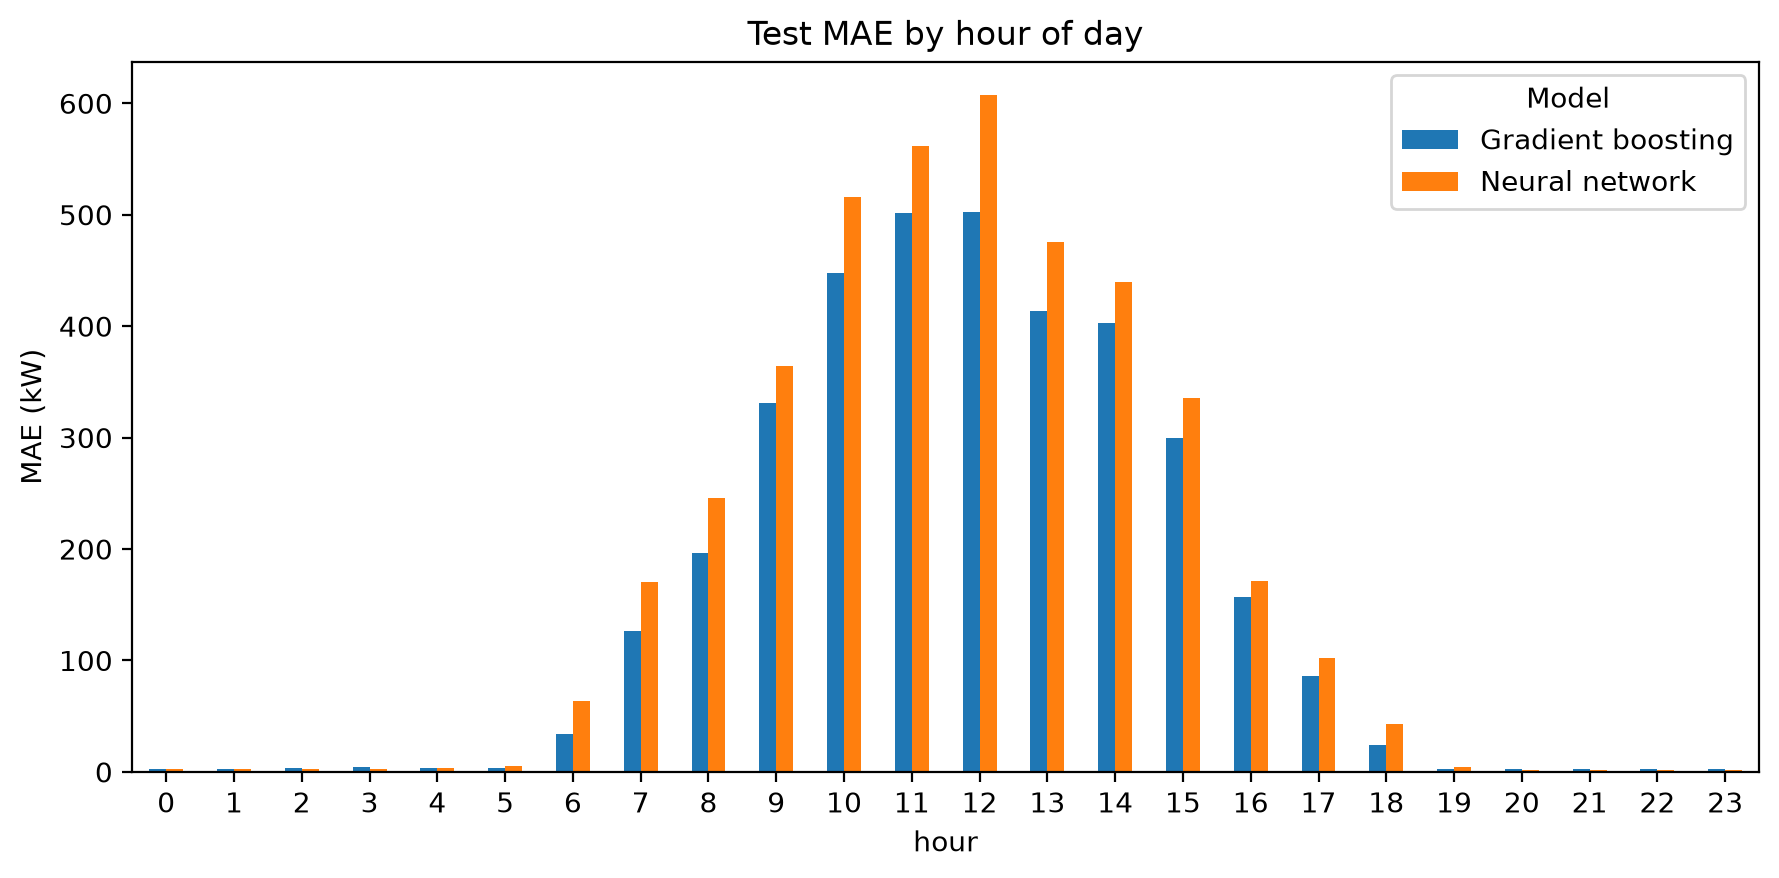
\includegraphics[width=0.85\textwidth]{error_by_hour.png}
\caption{Test error by hour of the day for both models.}
\label{fig:errhour}
\end{figure}

\subsection{Error by sunlight level}
Table~\ref{tab:irr} groups the test rows by the sunlight measured at the plant. The MAE grows with the sunlight level, but as a share of the mean output it stays at about 4 to 5\% for gradient boosting and 5 to 7\% for the neural network in all daytime bands. The models therefore do not get relatively worse in weak or strong sun; the absolute error grows because the output grows. The weakest daytime band has the highest relative error for the neural network (7.1\%).

\begin{table}[H]
\centering
\small
\begin{tabular}{lrrrrrr}
\toprule
\textbf{Sunlight (kW/m\textsuperscript{2})} & \textbf{Rows} & \textbf{Mean output} & \textbf{GB MAE} & \textbf{GB \%} & \textbf{NN MAE} & \textbf{NN \%} \\
\midrule
0 (night) & 4,541 & 0 & 2.96 & -- & 2.87 & -- \\
0--0.2 & 1,739 & 1,055 & 50.24 & 4.8 & 75.01 & 7.1 \\
0.2--0.5 & 1,750 & 5,023 & 245.43 & 4.9 & 285.65 & 5.7 \\
0.5--0.8 & 1,565 & 8,640 & 458.53 & 5.3 & 509.08 & 5.9 \\
$>0.8$ & 712 & 11,762 & 470.68 & 4.0 & 557.89 & 4.7 \\
\bottomrule
\end{tabular}
\caption{Test MAE by sunlight level for gradient boosting (GB) and the neural network (NN). The \% columns give the MAE as a share of the mean output in that band.}
\label{tab:irr}
\end{table}

\subsection{Largest errors}
The largest errors are single events rather than a general weakness. The biggest one for both models is on 7 June 2020 at 12:45 for inverter 5 (Inv05): the sunlight was high (1.0~kW/m\textsuperscript{2}) and both models predicted about 12,600 to 12,700, but the inverter produced only 3,770. Another large overprediction is Inv19 at 13:45 on the same day (actual 572, gradient boosting 7,043). In such cases the inputs say ``strong sun'' but the inverter output was low, so a model that only sees weather and time cannot predict the drop. Possible causes are an inverter fault, shading or a power limit, but the data does not say which.

The largest underpredictions go the other way. On 1 June 2020 at 11:15, several inverters (Inv03, Inv09 and Inv02) produced much more than predicted while the sensor showed only 0.49~kW/m\textsuperscript{2}, which suggests that the sensor reading at that moment did not match the sunlight reaching the panels. Several of the worst errors fall on the same timestamps and affect more than one inverter, which points to events in the plant or the sensor rather than to a weakness of one model.

\section{Bias Check}
The guide asks whether the model struggles with some groups. In the Kaggle data, the groups we can examine are the 22 inverters and the two months in the test set. We cannot check cities, because the Kaggle plant has no city column (see the Limitations section).

\subsection{By inverter}
Figure~\ref{fig:errinv} shows the MAE of each inverter. For gradient boosting it ranges from 98 (Inv10) to 210 (Inv07), a factor of about two. As a share of each inverter's mean output the range is smaller, 3.6\% to 6.5\%. The hardest inverters are the same for both models (Inv07 and Inv03 have the highest MAE for both, and Inv10 has the lowest for both), which suggests that the difference comes from the inverters' data and not from one model. The inverters also differ in how much they produce: the mean test output ranges from 2,692 (Inv12) to 3,595 (Inv03), even though all of them share the same weather. The model only knows an inverter through its ID, so differences between panel groups can only be learned through that ID.

The signed bias per inverter is small. For gradient boosting the largest is $+56$ for Inv19, which is 1.7\% of that inverter's mean output; for the neural network it is $-95$ for Inv21 (3.2\%). Inv19 is overpredicted by both models ($+56$ and $+59$) and appears several times in the list of largest errors, so it is the one inverter that deserves a closer look in the plant data.

\begin{figure}[H]
\centering
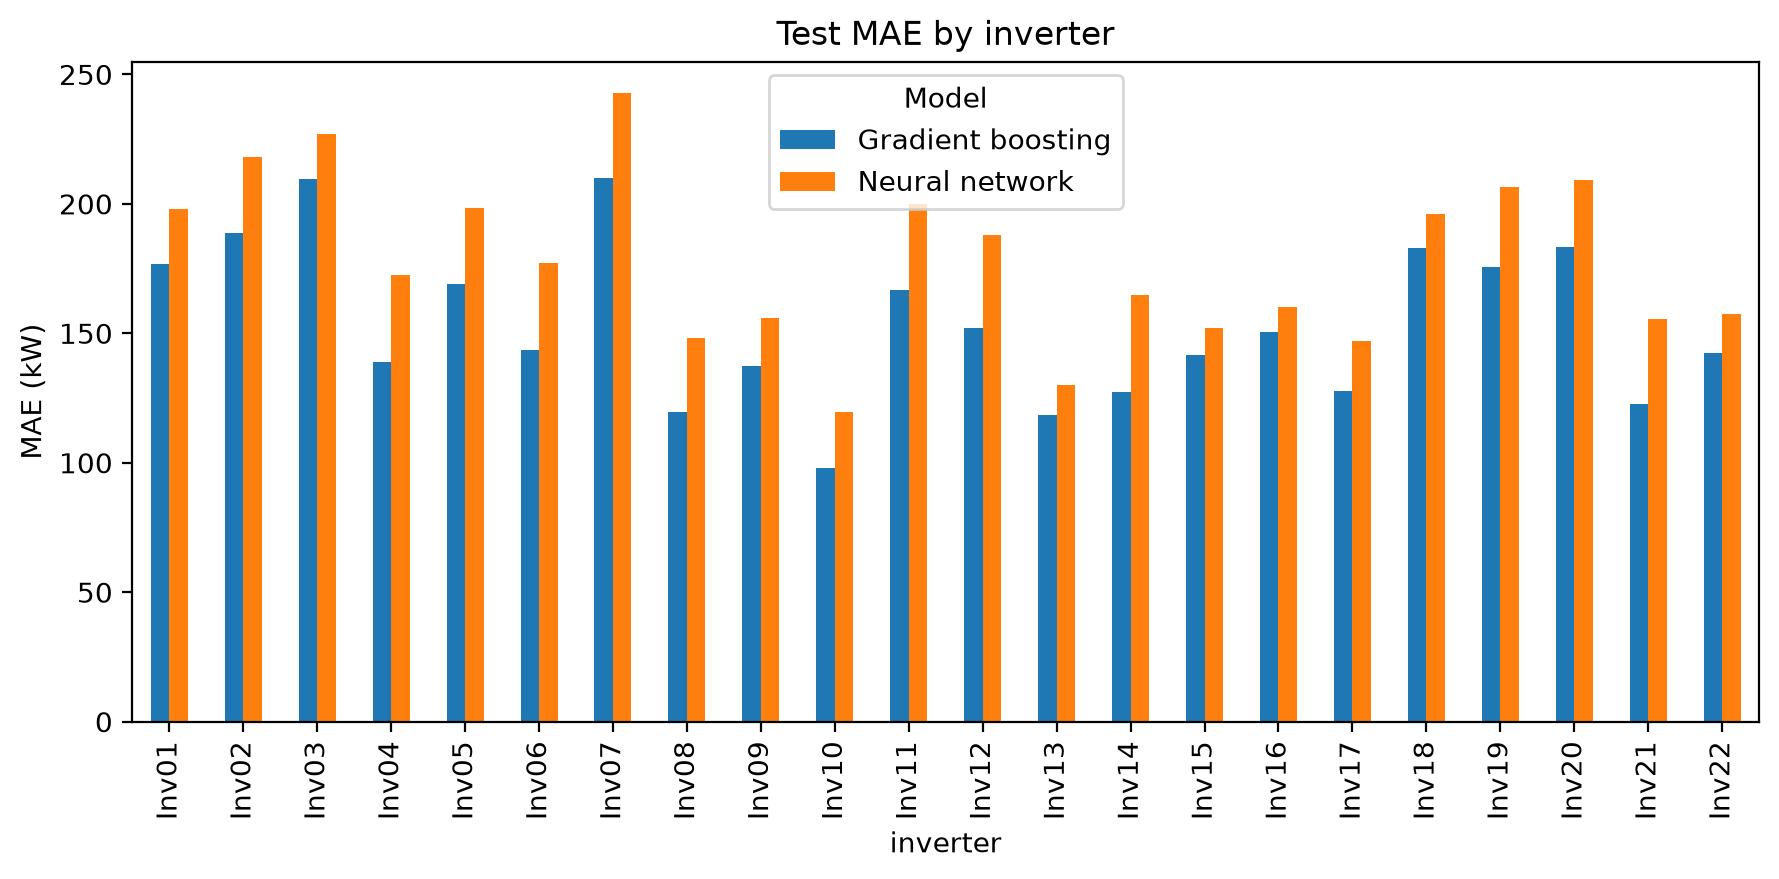
\includegraphics[width=\textwidth]{error_by_inverter.png}
\caption{Test MAE for each of the 22 inverters.}
\label{fig:errinv}
\end{figure}

\subsection{By month}
Only May and June 2020 appear in the data, so the month comparison has two groups (Figure~\ref{fig:errmonth}). For gradient boosting the MAE is 170.59 in May and 137.89 in June; for the neural network it is 196.84 and 161.10. May has the higher mean output (3,358 against 2,968), and as a share of the mean output the errors are similar: 5.1\% and 4.6\% for gradient boosting, 5.9\% and 5.4\% for the neural network. The bias is close to zero for gradient boosting ($+0.3$ and $+6.3$) and slightly negative for the neural network ($-32$ and $-22$).

\begin{figure}[H]
\centering
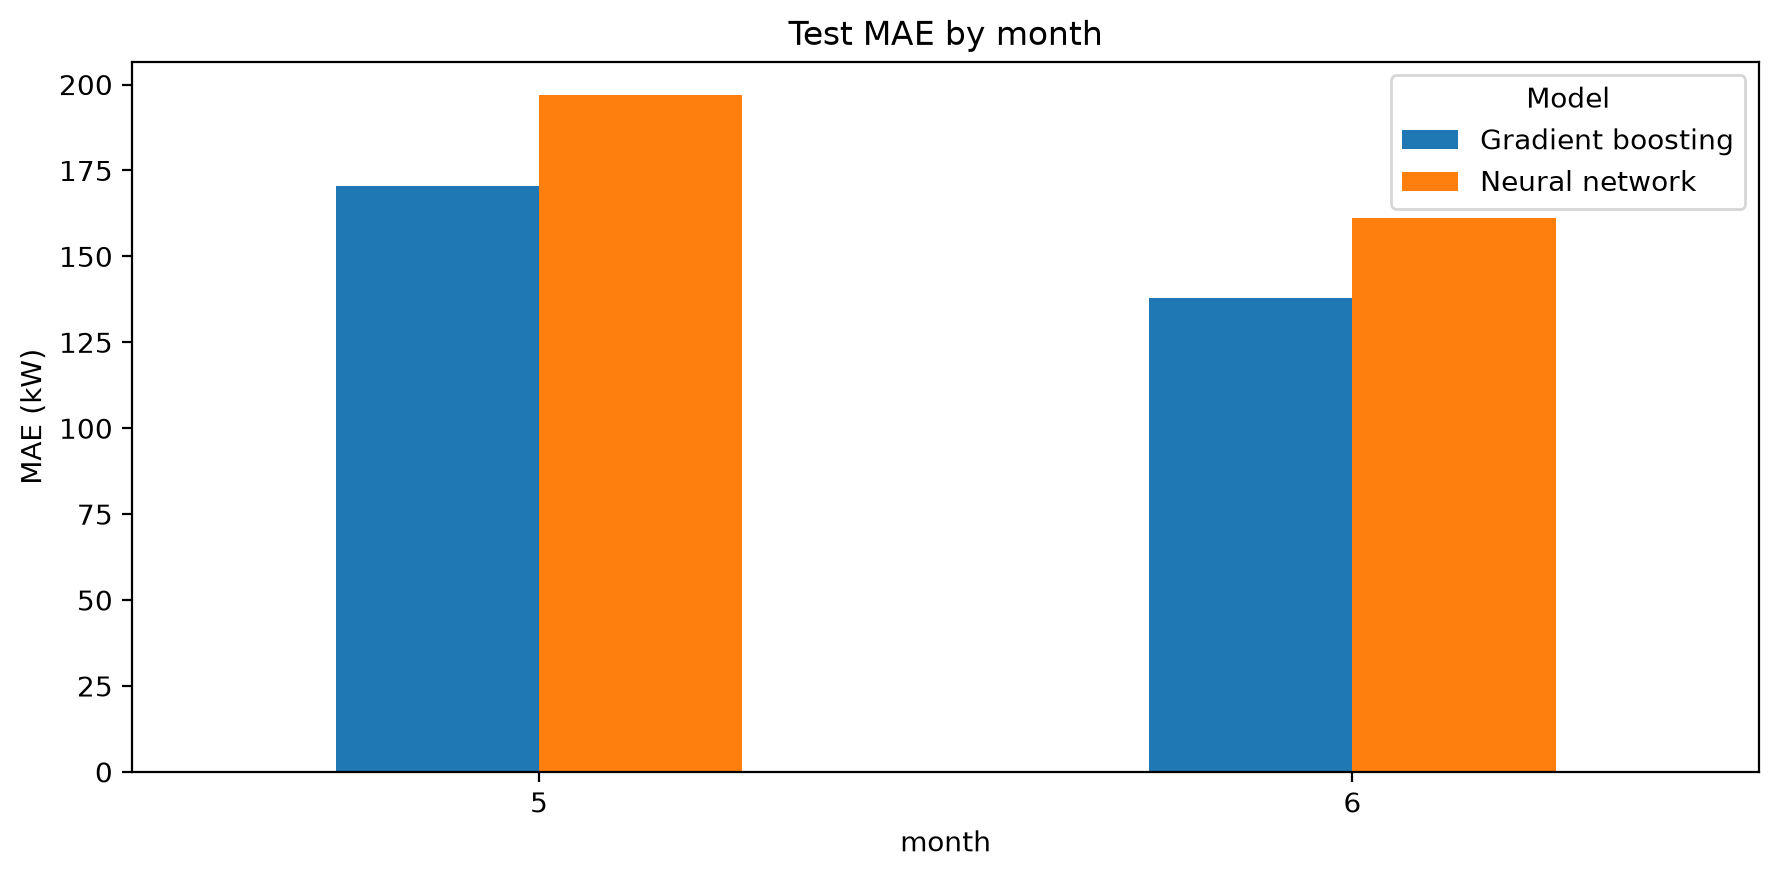
\includegraphics[width=0.7\textwidth]{error_by_month.png}
\caption{Test MAE by month for both models.}
\label{fig:errmonth}
\end{figure}

\subsection{Summary of the bias check}
We found no serious bias against any group we could test. No inverter is badly served: the signed bias per inverter is at most 1.7\% (gradient boosting) and 3.2\% (neural network) of its mean output. The two months have similar relative errors. The one systematic pattern is that the neural network underpredicts by about 1\% on average, while gradient boosting does not. Two limits apply: the data covers only two months, so we cannot say how the models behave in winter, in the monsoon or under heavy smog, and we have no test for differences between cities.